\chapter{Xử Lý Dữ Liệu Với NumPy Và Pandas \\ (NumPy \& Pandas)}

Trong khoa học dữ liệu và học máy, việc xử lý dữ liệu đóng vai trò nền tảng. Dữ liệu thực tế thường lộn xộn, thiếu sót hoặc không đúng định dạng. Để giải quyết vấn đề này, Python cung cấp hệ sinh thái các thư viện mạnh mẽ, trong đó nổi bật nhất là NumPy và Pandas. Chương này sẽ hướng dẫn bạn cách sử dụng hai thư viện này để thực hiện các thao tác tiền xử lý, phân tích và biến đổi dữ liệu một cách hiệu quả.

\section{Thư viện NumPy - Tính toán Khoa học}

NumPy (Numerical Python) là thư viện cốt lõi cho tính toán khoa học trong Python. Nó cung cấp đối tượng mảng đa chiều hiệu suất cao và các công cụ để làm việc với các mảng này.

\subsection{Khởi tạo mảng và kiểm tra thuộc tính}

NumPy hỗ trợ tạo mảng đa chiều từ list của Python hoặc sử dụng các hàm có sẵn để khởi tạo các ma trận đặc biệt.

\begin{lstlisting}[language=Python]
import numpy as np

arr1D = np.array([1, 2, 3, 4, 5, 6, 7, 8, 9, 10])
print("Shape 1D:", arr1D.shape, "| Dtype:", arr1D.dtype)

arr2D = np.array([[1, 2, 3, 4], 
                  [5, 6, 7, 8], 
                  [9, 10, 11, 12]])
print("Shape 2D:", arr2D.shape, "| So chieu (ndim):", arr2D.ndim)


arr_zeros = np.zeros((3, 4))
arr_ones = np.ones((2, 5))
arr_eye = np.identity(3)
arr_random = np.random.randn(3, 4)
\end{lstlisting}

\begin{figure}[H]
    \centering
    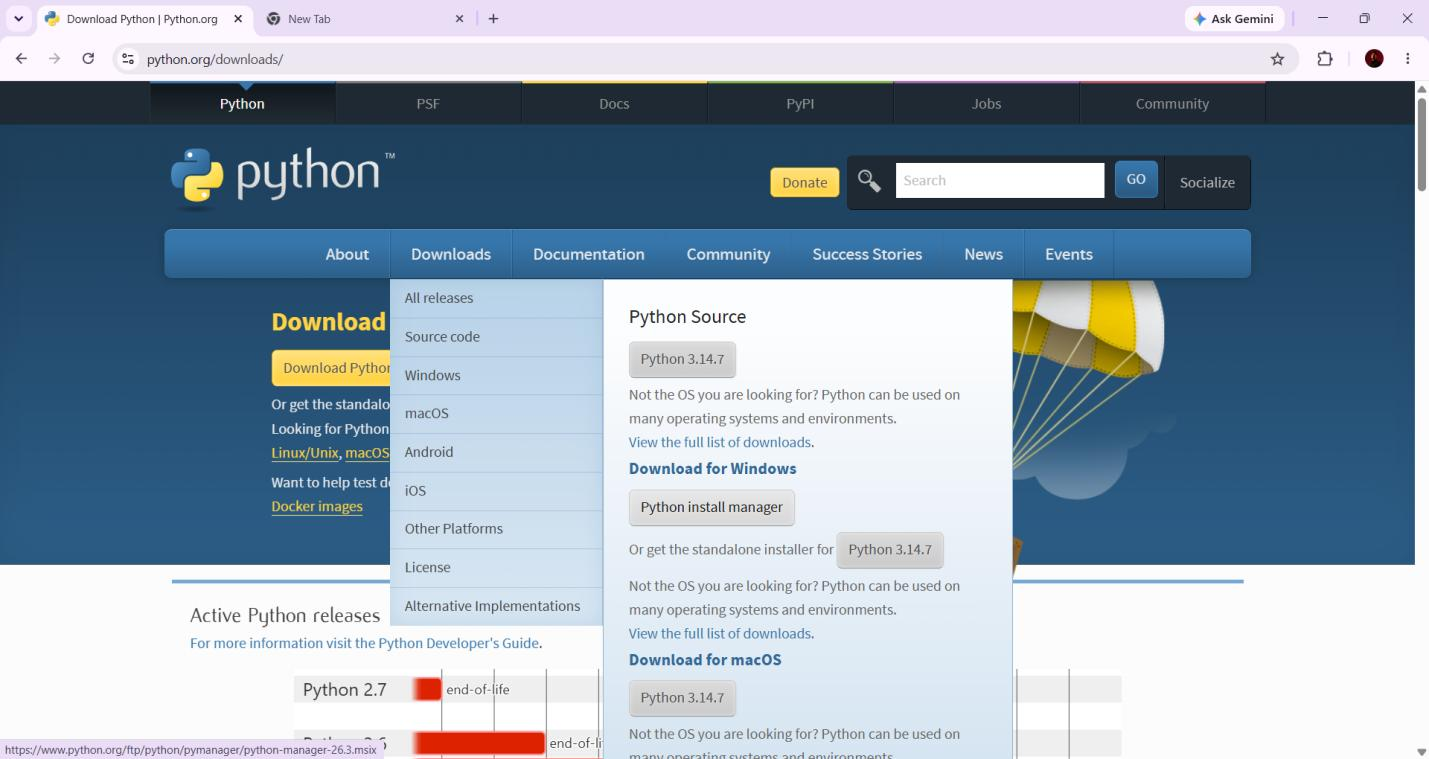
\includegraphics[width=0.8\textwidth]{images/B1.jpg}
    \caption{Khởi tạo và kiểm tra thuộc tính mảng NumPy}
    \label{fig:numpy_init}
\end{figure}

\subsection{Thao tác trên mảng: Thêm phần tử, xóa, sửa}

Trong quá trình xử lý, việc thay đổi cấu trúc mảng bằng cách thêm, xóa, sửa phần tử là rất thường xuyên. NumPy cung cấp các hàm như \texttt{append}, \texttt{insert}, và \texttt{delete} để thao tác với phần tử mảng.

\begin{lstlisting}[language=Python]
arr1D[0] = 99 

arr_appended = np.append(arr1D, [11, 12]) 
arr_inserted = np.insert(arr1D, 2, 999)  

arr_deleted = np.delete(arr1D, 0)       
\end{lstlisting}

\subsection{Slicing và Boolean Indexing (Lọc dữ liệu)}

Slicing cho phép lấy một phần của mảng, trong khi Boolean Indexing cho phép lọc các phần tử thỏa mãn điều kiện nhất định.

\begin{lstlisting}[language=Python]

sub_arr = arr2D[:2, :3]
print("Cat mang [:2, :3]:\n", sub_arr)


city_data = np.random.randn(5, 3)  
pos_values = city_data[city_data > 0]
print("Cac gia tri > 0:", pos_values)

city_data[city_data > 0] = 0
print("Ma tran sau khi thay the:\n", city_data)
\end{lstlisting}

\subsection{Đại số tuyến tính (Linear Algebra)}

NumPy tích hợp thư viện \texttt{linalg} cung cấp các hàm mạnh mẽ cho đại số tuyến tính như tính tích ma trận, ma trận nghịch đảo, giải hệ phương trình tuyến tính, v.v.

\begin{lstlisting}[language=Python]
A = np.array([[7, 5, -3], 
              [3, -5, 2], 
              [5, 3, -7]])
b = np.array([16, -8, 0])


x = np.linalg.solve(A, b)
print("Nghiem x, y, z:", x)
print("Kiem tra nghiem dung:", np.allclose(np.dot(A, x), b))
\end{lstlisting}

\section{Thư viện Pandas - Xử lý và Phân tích Dữ liệu}

Pandas được xây dựng dựa trên NumPy, cung cấp các cấu trúc dữ liệu linh hoạt là \texttt{Series} (1D) và \texttt{DataFrame} (2D), đặc biệt phù hợp cho dữ liệu dạng bảng.

\subsection{Tạo và Đọc dữ liệu}

Pandas cung cấp hàm \texttt{read\_csv()} để đọc dữ liệu từ tệp CSV và các hàm như \texttt{head()}, \texttt{tail()} để quan sát dữ liệu. Ngoài ra, ta có thể khởi tạo DataFrame từ Dictionary hoặc List.

\begin{lstlisting}[language=Python]
import pandas as pd

data_dict = [
    {'city': 'Delhi', 'data': 1000},
    {'city': 'Bangalore', 'data': 2000},
    {'city': 'Mumbai', 'data': 1500}
]
df_dict = pd.DataFrame(data_dict)

data_list = [[1, 'Apple'], [2, 'Banana']]
df_list = pd.DataFrame(data_list, columns=['ID', 'Fruit'])

data_vnm = {
    'Date': ['10-01-2023', '10-02-2023', '10-03-2023', '10-04-2023', '10-05-2023', '10-06-2023', '10-07-2023'],
    'Ticker': ['VNM', 'VNM', 'VNM', 'VNM', 'VNM', 'VNM', 'VNM'],
    'Open': [75.5, 76.0, 75.8, 77.2, 76.5, 78.0, 77.8],
    'Close': [76.0, 75.5, 77.0, 76.5, 78.0, 77.5, 78.2],
    'Volume': [12000, 15000, 13500, 18000, 16000, 20000, 19500]
}
df_mock = pd.DataFrame(data_vnm)


df_mock.to_csv('vinamilk_stock.csv', index=False)
print("Đã tạo thành công file 'vinamilk_stock.csv' trong thư mục hiện tại!")

df_stock = pd.read_csv('vinamilk_stock.csv')

print("--- 5 DONG DAU CUA DU LIEU ---")
print(df_stock.head()) 

print("\n--- 3 DONG CUOI CUA DU LIEU ---")
print(df_stock.tail(3)) 
\end{lstlisting}

\begin{figure}[H]
    \centering
    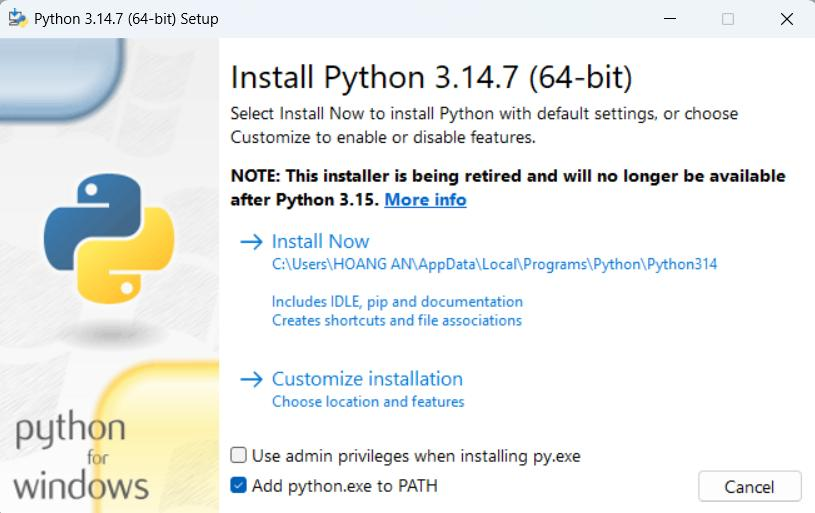
\includegraphics[width=0.8\textwidth]{images/B2.jpg}
    \caption{Tạo và Đọc dữ liệu với Pandas}
    \label{fig:pandas_init}
\end{figure}

\subsection{Truy xuất \& Điều kiện lọc dữ liệu}

Hai thuộc tính quan trọng để truy cập dữ liệu trong Pandas là \texttt{loc} (theo nhãn) và \texttt{iloc} (theo vị trí số nguyên).

\begin{lstlisting}[language=Python]
data_fict = {
    'price': [100, 200, 300],
    'quantity_purchased': [10, 20, 32],
    'user_type': ['A', 'B', 'C'],
    'user_class': ['X', 'Y', 'Z']
}
df = pd.DataFrame(data_fict)
print(df.iloc[:5, :4])
df_filtered = df.loc[df['quantity_purchased'] > 25]
\end{lstlisting}

\subsection{Xử lý dữ liệu khuyết \& Thống kê mô tả}

Pandas cung cấp các công cụ để phát hiện và xử lý dữ liệu bị thiếu (\texttt{NaN}) cũng như các hàm để mô tả nhanh bộ dữ liệu như \texttt{describe()} hay \texttt{info()}.

\begin{lstlisting}[language=Python]
print(df.describe())

mean_price = df['price'].mean()
df['price'].fillna(value=mean_price, inplace=True)
\end{lstlisting}

\subsection{Thay thế và Áp dụng hàm}

Các phương thức \texttt{replace()} và \texttt{apply()} là những công cụ mạnh mẽ để thay đổi hoặc biến đổi dữ liệu trên cột.

\begin{lstlisting}[language=Python]
df['user_type'] = df['user_type'].replace({'A': 'Premium', 'B': 'Standard'})

df['discounted_price'] = df['price'].apply(lambda x: x * 0.9)
\end{lstlisting}

\subsection{Gom nhóm (GroupBy) \& Gộp dữ liệu (Concat/Merge)}

Hàm \texttt{groupby()} rất hữu ích để nhóm các dòng theo giá trị của một cột và thực hiện các phép toán thống kê.

\begin{lstlisting}[language=Python]
grouped = df.groupby('user_class')['quantity_purchased'].agg(['sum', 'mean', 'count'])
print(grouped)
\end{lstlisting}

